\documentclass[runningheads]{llncs}
% cmap must precede fontenc: fixes ToUnicode so fi/fl/ff can be copied,
% searched and indexed (otherwise they extract as (cid:28) and break the
% similarity check).
\usepackage{cmap}
\usepackage[T1]{fontenc}
\usepackage[utf8]{inputenc}
\input{glyphtounicode}
\pdfgentounicode=1
\usepackage[english]{babel}
\usepackage{amsmath,amsfonts,amssymb}
\usepackage{graphicx}
% Mapa1.png y Mapa2.png viven en Imagenes/, pero se citan por su nombre a
% secas: compilando desde esta carpeta LaTeX no las encontraba y las
% sustituia por cajas vacias, lo que ademas anadia una pagina. Se buscan
% primero en Imagenes/ y luego junto al .tex, asi funciona tanto con el
% arbol actual como con un envio plano a la editorial.
\graphicspath{{Imagenes/}{./}}
\usepackage{subcaption}
\usepackage{xcolor}
\usepackage{booktabs}
\usepackage{array}
\newcolumntype{L}[1]{>{\raggedright\arraybackslash}p{#1}}
\usepackage{float}
\usepackage{tikz}
\usetikzlibrary{arrows.meta,positioning,shapes.geometric,fit,backgrounds,calc}
\usepackage{tabularx}
\usepackage{listings}
\usepackage{hyperref}
\usepackage{url}
\newcolumntype{Y}{>{\raggedright\arraybackslash}X}

% =====================================================================
%  CAMBIOS DE LA VERSION ICOKG 2026 RESPECTO A LA ENVIADA A REVISION
%  \icokg{...} y el entorno icokgblock marcan en AZUL lo nuevo o
%  reescrito para atender a los revisores.
%  Para el PDF final: \marcarcambiostrue -> \marcarcambiosfalse
% =====================================================================
\definecolor{nuevo}{RGB}{0,84,166}
\newif\ifmarcarcambios
\marcarcambiosfalse
\newcommand{\icokg}[1]{\ifmarcarcambios\textcolor{nuevo}{#1}\else#1\fi}
\newenvironment{icokgblock}{\ifmarcarcambios\color{nuevo}\fi}{}

% =====================================================================
%  VERSION EXTENDIDA PARA IJCOPI (numero especial ICOKG 2026)
%  Fuente de la version que se envia a la revista; dw_agua_icokg2026.tex
%  es el camera-ready de Springer y no se modifica.
%  \nuevo{...} y el entorno nuevobloque marcan lo que cambia respecto al
%  camera-ready; paper/ijcopi/latex_a_ijcopi.py lo resalta en AMARILLO en
%  el Word, como pide el numero especial. Las referencias nuevas se marcan
%  con "!" en REFERENCIAS dentro del conversor.
% =====================================================================
\newcommand{\nuevo}[1]{\colorbox{yellow}{#1}}
\newenvironment{nuevobloque}{}{}

\lstdefinestyle{ttl}{basicstyle=\ttfamily\scriptsize,breaklines=true,
  columns=fullflexible,keepspaces=true,frame=single,framesep=3pt,
  xleftmargin=3pt,aboveskip=5pt,belowskip=3pt}
\lstset{style=ttl}

\hypersetup{colorlinks=true,linkcolor=blue,urlcolor=blue,citecolor=blue}
\def\UrlBreaks{\do\/\do-\do_\do.}
\emergencystretch=3em
% interlineado: valor por defecto de LNCS
% Colocacion de flotantes: evita paginas a medio llenar (Reviewer #4)
\setcounter{topnumber}{3}\setcounter{bottomnumber}{2}\setcounter{totalnumber}{4}
\renewcommand{\topfraction}{0.92}\renewcommand{\bottomfraction}{0.75}
\renewcommand{\textfraction}{0.06}\renewcommand{\floatpagefraction}{0.80}
% Line breaks in underscore identifiers (avoids margin overflow)
\let\origunderscore\_
\renewcommand{\_}{\origunderscore\allowbreak}

\begin{document}


\title{Territorial Information Retrieval from Heterogeneous Open Data\nuevo{: Extending a Water Data Warehouse from Mexico City to its Metropolitan Area}}
\titlerunning{Extending a Water Data Warehouse to the Mexico City Metropolitan Area}

\author{%
Gabriel Hurtado Avil\'es\thanks{Corresponding author: \href{mailto:gabrielhuav@gmail.com}{gabrielhuav@gmail.com}}\orcidID{\href{https://orcid.org/0009-0002-5686-1822}{0009-0002-5686-1822}} \and
Roberto Eswart Zagal Flores\orcidID{\href{https://orcid.org/0000-0001-5649-6189}{0000-0001-5649-6189}} \and
Eduardo Uriel Vel\'azquez Arrieta\orcidID{\href{https://orcid.org/0009-0001-8745-2717}{0009-0001-8745-2717}} \and
% ORCID enlazados a orcid.org. Desde llncs 2.24 \orcidID se compone en modo texto, asi que la X va
% cursiva matematica y al copiarla del PDF da U+1D44B en vez de X: el ORCID
% quedaria roto. \mathrm{X} la deja recta y copiable.
Omar Fernando Pulido Morales\orcidID{\href{https://orcid.org/0009-0001-5698-987X}{0009-0001-5698-987X}} \and
Emilio Garc\'ia L\'opez\orcidID{\href{https://orcid.org/0009-0005-2550-0671}{0009-0005-2550-0671}} \and
Clara Aide Hern\'andez Mart\'inez\orcidID{\href{https://orcid.org/0009-0008-0647-8458}{0009-0008-0647-8458}}%
}
\authorrunning{G. Hurtado Avil\'es et al.}
\institute{\icokg{Escuela Superior de C\'omputo (ESCOM),} Instituto Polit\'ecnico Nacional, Mexico City, Mexico\\
\email{\{evelazqueza1900,opulidom2000,egarcial2001,chernandezm1903\}@alumno.ipn.mx}\\
\email{ghurtadoa@ipn.mx, rzagalf@ipn.mx}\\
% Correos personales, en el mismo orden de firma. Van en dos lineas: en una
% sola, la linea se sale del margen 26pt.
\email{velazquez.arrieta.uriel@gmail.com, pulido.morales.omar@gmail.com}\\
\email{egarlo@hotmail.com, claraahm11@gmail.com, gabrielhuav@gmail.com}}

\maketitle

\begin{abstract}
This work presents a data warehouse for the territorial information retrieval of water consumption in Mexico City, built from heterogeneous open sources\nuevo{ and extended to its metropolitan area}. The contribution lies in three elements: an ETL process that consolidates SACMEX data into a dimensional model of 70,886 records, a declarative R2RML mapping that republishes the star schema as an RDF knowledge graph, and a static deployment methodology. \nuevo{Against the 2020 Census, billed volumes amount to 47 litres per inhabitant per day, 38\,\% of published consumption, least in the periphery, and the atypical-consumption score structurally misses drops. The extension integrates 62 verified files on 63 municipalities into 2.79 million rows and a metropolitan knowledge graph: municipal volumes require a quality filter, and neighbourhoods with almost no billed volume report shortages nearly as often as the rest. Every map layer is a verified SQL query.}
\end{abstract}

\keywords{Data warehouse, Open data, Knowledge graph, RDF Data Cube, Water consumption, \nuevo{Anomaly detection}}

\section{Introduction}

Mexico City faces a water crisis of aquifer overexploitation, network leaks and population growth. Open data on water consumption exist (SACMEX), but in poorly accessible formats and without query tools, which limits their use for evidence-based decision making.

This work addresses the problem from two perspectives proper to information processing: the extraction of structured information from heterogeneous open sources through an ETL process, and the retrieval of that information through a parameterized query interface, transforming dispersed datasets into a queryable dimensional repository that anyone can filter and visualize geospatially by \nuevo{neighbourhood} and borough.

The contribution of this work is \icokg{threefold}: (i) a reproducible ETL process to consolidate official open data into a dimensional data warehouse, \icokg{(ii) a declarative R2RML mapping that republishes it as a validated RDF knowledge graph,} and \icokg{(iii)} a continuous-deployment methodology that keeps a functional demonstration always accessible, combining a dynamic deployment connected to a database with a static version published in a public repository.

The analysis of the 70,886 consolidated records reveals that the boroughs of Cuauht\'emoc and Miguel Hidalgo lead the total consumption (Table~\ref{tab:top5_alcaldias}), and that consumption varies across the available bimesters without a direct causal relationship with dry or rainy periods. \icokg{The system serves citizens querying their own neighbourhood, public servants diagnosing territorial demand, researchers, journalists and civil organisations monitoring water management.}

\begin{nuevobloque}
This article extends the version presented at ICOKG 2026~\cite{velazquez2026icokg}. It adds an
account of what a consumption value in the source actually is (Section~\ref{sec:grain}); a measure,
against the 2020 Census, of how much of the city's consumption the billed volumes represent and of
how the borough ranking changes per inhabitant (Section~\ref{sec:percapita}); a sensitivity analysis
showing that the deployed atypical-consumption statistic is structurally blind to drops
(Section~\ref{sec:sens}), with a diagnosis on the real data (Section~\ref{sec:real}); and the
extension of the warehouse to the metropolitan area, published in a map whose layers are verified
SQL queries and in a knowledge graph that crosses the city boundary (Sections~\ref{sec:metro}
and~\ref{sec:kgmetro}).
\end{nuevobloque}

Section~\ref{sec:edo} reviews related work, Section~\ref{sec:met} describes the methodology, Section~\ref{sec:res} presents the results and Section~\ref{sec:con} the conclusions.

\section{Related Work}
\label{sec:edo}

\subsection{Foundations: Data Warehouses, Dimensional \nuevo{Modelling}, and ETL}

Dimensional \nuevo{modelling} and the star schema constitute the consolidated basis for the design of analytical data warehouses. Kimball and Ross~\cite{kimball} establish the canonical principles ---fact and dimension tables, surrogate keys, slowly changing dimensions, and the ETL subsystems--- that ground the model adopted in this work. On the integration phase, Vassiliadis~\cite{vassiliadis2009} offers a reference survey of \emph{Extract--Transform--Load} technology, covering the conceptual and logical \nuevo{modelling} of the processes and the cross-cutting extraction, transformation, and loading issues that methodologically support our pipeline.

\subsection{Data Warehouses and Information Systems for Water Management}

In the water domain, the most direct antecedent is that of Soares et al.~\cite{soares2019}, who implement a data warehouse with an ETL process to monitor water supply and consumption, integrating meter readings, reservoir volumes, and geographic location from management-application databases and heterogeneous files. Abecker et al.~\cite{abecker2014} present a hybrid sensor-semantic architecture (the WatERP project) that combines a relational/PostGIS store with a triple store for integrated resource management. These systems, however, mostly start from operational data, SCADA, or proprietary sensor networks, and not from open government data.

\begin{nuevobloque}
\subsection{Water Consumption in Mexico City from Utility Records}

Peer-reviewed spatial analyses of consumption in Mexico City come mainly from two
groups, and both obtained their data from the utility rather than from the open
portal. Medina-Rivas et al.~\cite{medina2022} analyse the 2019 records, the year
of the open export used here, report a domestic consumption of 123 litres per
person per day, and find two clusters of unequal consumption explained by
discontinuous supply, dependence on external sources, altitude and socioeconomic
status; a later study finds that per-capita domestic use fell by 40\,\% between
2010 and 2019 while its spatial distribution became more unequal~\cite{medina2025}.
Ramos-Bueno et al.~\cite{ramosbueno2021} obtained colonia-level consumption and
metering for 2008--2013 through public-information requests and explain
residential demand with spatial regression, after excluding colonias with zero
consumption or no metering coverage, and a panel study by the same group extends
the series to 2004--2022~\cite{ramosbueno2024}. These works answer substantive
questions with data a reader cannot obtain from the portal. The present one
addresses the complementary problem of making the open export itself queryable
and verifiable, and what it finds about the billing basis and about colonias
without billed volume (Sections~\ref{sec:grain} and~\ref{sec:real}) is consistent
with the exclusions those studies apply. Closer in method, Hern\'andez-V\'azquez et
al.~\cite{hernandez2026} fuse SACMEX, INEGI and DENUE data in a GIS, with a layered
architecture for historic data, and cluster consumption from boroughs to
neighbourhoods, and Daowz Laguna et al.~\cite{daowz2027} use large language models
to turn citizen reports from social media and the web into features for analysing
leak incidents. Both aim at spatial analysis; this work aims at a dimensional
warehouse and a knowledge graph over the open sources.
\end{nuevobloque}

\subsection{The Gap: ETL over Heterogeneous Open Data and Data Quality}

Integrating open government data into dimensional warehouses poses its own challenges. Berro, Megdiche, and Teste~\cite{berro2015} propose ``content-driven'' ETL processes that address precisely the semantic and structural heterogeneity, the absence of schemas, and the dispersion characteristic of open data, factors that overwhelm traditional ETL. Complementarily, Vetr\`o et al.~\cite{vetro2016} define a quantitative measurement framework for the quality of Open Government Data (accuracy, completeness, consistency, traceability, and freshness) and empirically report that the most frequent problems are missing metadata, incomplete data, and the absence of update information ---exactly the challenges our ETL faces over the SACMEX data.

\subsection{Geospatial Information Retrieval and Visualization}

Purves et al.~\cite{purves2018} offer a reference monograph on Geographic Information Retrieval (GIR) ---indexing, search, and spatial ranking--- that theoretically frames the territorial information-retrieval component of this work.

\begin{icokgblock}
\subsection{Knowledge Graphs for Urban and Water Domains}

Republishing a relational warehouse as RDF is a mature practice with W3C
standards for both ends. The RDF Data Cube vocabulary~\cite{datacube} models
statistical observations over conformed dimensions, which is the same structure a
star schema encodes; R2RML~\cite{r2rml} specifies the mapping declaratively, so
the graph is derived rather than maintained by hand; and GeoSPARQL~1.1, documented by Car and
Homburg~\cite{carhomburg2022}, supplies the geometry model and the topological
vocabulary that a flat territorial dimension cannot express. In the
water and urban domains the direction is established: Roussey et
al.~\cite{roussey2023} survey knowledge-graph technologies as the next frontier
for food, agriculture and water. \nuevo{The closest graph in the water domain is
the Water Health Open Knowledge Graph~\cite{lippolis2025}, built in a European
project, which models water consumption together with pollution, extreme weather,
infectious disease and drug distribution; we found no RDF knowledge graph built
over Mexican utility water data.} What these works share is the premise this
article adopts: the graph is valuable for interoperability and topological
querying, not as a replacement for the analytical store.
\end{icokgblock}

\subsection{Reproducibility and Deployment of Scientific Demonstrations}

Finally, Sandve et al.~\cite{sandve2013} formulate widely cited rules for computational reproducibility (version control, documentation of preprocessing, public access to data and scripts) that ground our reproducible static version. Hill et al.~\cite{hill2023} provide a practical guide to developing and deploying an open-source, reproducible web dashboard for water-sanitation data, a close domain that supports the continuous-deployment methodology with reproducible \nuevo{artefacts}.

\subsection{Positioning of the Contribution}

Unlike existing water data warehouses ---which start from operational data, SCADA, or proprietary sensors~\cite{soares2019,abecker2014}--- and recognizing that the integration of heterogeneous open data is a documented but unsolved problem in this domain~\cite{berro2015,vetro2016}, this work differs in three respects. First, an ETL process designed to consolidate official SACMEX open data into a dimensional star schema. Second, \icokg{the exposure of the information through parameterized queries and a choropleth geospatial visualization that enables territorial information retrieval~\cite{purves2018}, published as static artefacts that require no server}. Third, a continuous-deployment methodology accompanied by a reproducible static version that guarantees the indefinite verifiability of the system~\cite{sandve2013,hill2023}. This same approach of consolidating official open data was previously applied to the seismic-risk domain in Mexico~\cite{villa2026}, a direct methodological antecedent transferred here to the water domain. To the best of our review, no academic, peer-reviewed, and reproducible data warehouse built specifically over SACMEX/CDMX open data exists.

\section{Methodology}
\label{sec:met}

\subsection{General Architecture}

The system follows a layered architecture: a data layer (PostgreSQL), a processing layer (ETL with Python and SQL), \icokg{a query layer of parameterized SQL and, over it, a declarative RDF projection}, and a presentation layer (HTML/CSS/JS frontend with Leaflet and Plotly). The warehouse implements a star schema over \icokg{two fact tables ---\texttt{fact\_consumo\_agua}, the subject of this article, and \texttt{fact\_clima}, the climate series joined through the shared temporal dimension--- and three conformed dimensions: \texttt{dim\_tiempo} (date, year, bimester), \texttt{dim\_ubicacion} (borough, \nuevo{neighbourhood}, latitude, longitude) and \texttt{dim\_indice\_des} (development level). Identifiers are quoted verbatim from the published schema.}

\subsection{ETL Consolidation Process}

The first contribution of the work is the ETL process that consolidates the SACMEX open data into the dimensional warehouse. The complete detail of the process \icokg{---the DDL and the ETL scripts (\texttt{ddl/0\_schema.sql}, \texttt{etl/1\_copy.sql}, \texttt{etl/2\_dim.sql}, \texttt{etl/3\_fact.sql}) and the parameterized retrieval queries---} is documented in the project's public repository; this article presents only the architecture of the process.

The pipeline operates in four phases. (1) \textbf{Extraction}: reading the open SACMEX CSV files. (2) \textbf{Validation and cleaning}: discarding records with empty fields, inconsistent coordinates, or incompatible formats. (3) \textbf{Loading to staging and populating dimensions}: \texttt{COPY} of the data into temporary tables and extraction of the unique values into \icokg{\texttt{dim\_tiempo}, \texttt{dim\_ubicacion} and \texttt{dim\_indice\_des}}. (4) \textbf{Populating the fact tables}: a join between staging and dimensions \icokg{that populates \texttt{fact\_consumo\_agua} and \texttt{fact\_clima}}, finally dropping the staging tables. \icokg{The information thus consolidated becomes available for retrieval through the parameterized queries distributed with the archived release.}\footnote{SACMEX operates a proprietary platform integrating SCADA and multiple sources; it is distinguished from a reproducible academic work over open data such as this one.}


\subsection{Continuous Deployment Methodology}

So that the demonstration survives without a server, the system is published in
two modalities. The \textbf{dynamic deployment} keeps the complete architecture
\icokg{over PostgreSQL}, serves parameterized queries and produced the results
reported here. The \textbf{static version} exports the data as \texttt{JSON} and
\texttt{GeoJSON} that the frontend consumes directly, so querying, filtering,
aggregation and visualization run on the client.
\icokg{The duality addresses the recurring problem that academic prototypes stop
working shortly after evaluation~\cite{sandve2013,hill2023}.} The system is
available at \icokg{\url{https://github.com/gabrielhuav/Data_Warehouse_static}
(repository), \url{https://gabrielhuav.github.io/Data_Warehouse_static/} (static
demo, no backend required) and
\url{https://github.com/gabrielhuav/data_warehouse_cdmx} (warehouse,
preservation fork)}.

\begin{icokgblock}
\noindent What is preserved deserves precision. The archived release
(\url{https://github.com/gabrielhuav/Data_Warehouse_static/releases/tag/v1.5-icokg2026})
distributes the warehouse itself ---schema, ETL, both source files and the
container definition that rebuilds the database, vendored unmodified from its
author's repository and additionally preserved as a fork--- together with the
static frontend, the R2RML mapping, a browser-side SPARQL explorer
(\url{https://gabrielhuav.github.io/Data_Warehouse_static/grafo.html}) and the
scripts that regenerate the exported data, so the JSON the demonstration consumes
is an export of the warehouse and not a separate dataset. Citations refer to the
frozen release; the repository head may evolve, the release will not.

\subsection{Data Scope, Grain and Cleaning Criteria}
\label{sec:grain}

\nuevo{Four} properties of the source bound every result reported below.
\emph{Extent}: the resource is published as \emph{Consumo Agua (1er Semestre
2019)}\nuevo{~\cite{sacmex2026}} and contains exactly that ---the first three bimesters of 2019, one
reading date each, in 71,102 records--- so the warehouse is not a multi-year
series and the seasonal variation it supports is a within-semester comparison.
The bound is declared by the publisher in the title of the resource, not chosen
by us, \nuevo{and when the portal migrated the resource in August~2026 it still
held those three bimesters, identical in content to the file consolidated here
(same MD5, \texttt{41495b03\ldots}, once line endings are normalised)}: a partial
extraction published once, without versioning, which is the problem this article
studies. Against the source becoming unavailable, both files the ETL consumes are
redistributed with the archived release and the portal page is preserved in the
Internet Archive. \emph{Grain}: one fact row is one \emph{manzana} (city block)
for one billing period, and the export carries 22,930 distinct coordinate-bearing
units over 1,553 borough--neighbourhood pairs, so the location dimension is
coarser than the grain and every aggregate is a roll-up. \emph{Scale}: the
development index has four ordinal levels ---\textsc{alto}, \textsc{medio},
\textsc{bajo} and \textsc{popular}--- published with the dataset rather than
derived here.

\begin{nuevobloque}
\emph{Billing basis}: a consumption value is a billed volume, not a meter reading.
The clarifying note that the publisher distributes with the data dictionary,
grounded in the 2019 Fiscal Code of Mexico City, states that an intake is billed
by its meter where one is installed and authorised, and otherwise by an average:
the average of its cadastral \emph{colonia} when at least 70\,\% of the intakes
there are metered, or the average of the intake's last six metered bimesters when
its meter is broken or cannot be read. The export does not say which basis
applies to each record, so part of every aggregate is imputed by construction,
in a proportion the data do not reveal. Two consequences follow. A neighbourhood
with unusually uniform consumption may reflect averaging rather than uniform
behaviour, and a detector run on these values ranks departures in billing, which
coincide with departures in physical use only where intakes are metered. The same
note defines the \emph{manzana} as a cadastral unit, identified by digits of the
cadastral account number rather than by the census geography, so joining the
warehouse to census data requires a spatial join on the coordinates, not a key
match; and it defines the development index as a statistical construct over
socioeconomic variables aggregated to the block, which is why the knowledge graph
treats the four levels as an ordinal scale rather than as measured quantities.
\end{nuevobloque}

The exclusion criteria are deterministic and enforced structurally: the fact
table is populated by inner joins against the three dimensions, so a record that
fails to resolve a dimension member is not loaded. Table~\ref{tab:cleaning}
quantifies each criterion rather than merely declaring data
quality~\cite{vetro2016}. The distribution is unusually clean and that is itself
a finding: a single criterion accounts for every discarded record ---the 216 rows
carrying the literal \texttt{NA} in both territorial fields--- and none is lost
to a malformed measure or an unparseable date. This is a property of the SACMEX
export rather than a merit of the process.

\begin{table}[tbp]
\centering
\caption{Records discarded during validation and cleaning, over the 71,102
records of the source export.}
\label{tab:cleaning}
\begin{tabular}{lrr}
\hline
\textbf{Exclusion criterion} & \textbf{Records} & \textbf{\% of source} \\
\hline
Unmatched territorial label                 &    216 &  0.30 \\
Missing development index                   &      0 &  0.00 \\
Reading date absent from the time dimension &      0 &  0.00 \\
\hline
\textbf{Total discarded}                    &    216 &  0.30 \\
\textbf{Loaded into the fact table}         & 70,886 & 99.70 \\
\hline
\end{tabular}
\end{table}

\noindent\textbf{Data sources and attribution.} The meteorological series comes
from Open-Meteo under CC~BY~4.0 and the cartographic base of the interactive map
is OpenStreetMap under the Open Database License, which requires attribution
wherever the map is reproduced.
\end{icokgblock}

\subsection{Frontend and Geospatial Visualization}

The frontend offers a dashboard with indicators, interactive charts (Plotly), and
a choropleth map of the 16 boroughs (Leaflet + GeoJSON), where \nuevo{colour} represents
the consumption level and each borough displays a popup with its detail
(Fig.~\ref{fig:mapa-a}). \icokg{Alongside it, and over the same exported data, a
second view resolves territorial adjacency by traversing the knowledge graph of
Section~\ref{sec:kg} rather than by filtering the cube: selecting a neighbourhood
returns its neighbours ranked by consumption, together with the
\icokg{\texttt{agua:nearbyWithin1500m}} query that produced them (Fig.~\ref{fig:mapa-b}). The two
views in Fig.~\ref{fig:mapa} are therefore the same warehouse read through its
two representations, and both run in the browser with no server behind them.}

\begin{figure}[tbp]
\centering
\begin{subfigure}[t]{0.485\textwidth}
  \centering
  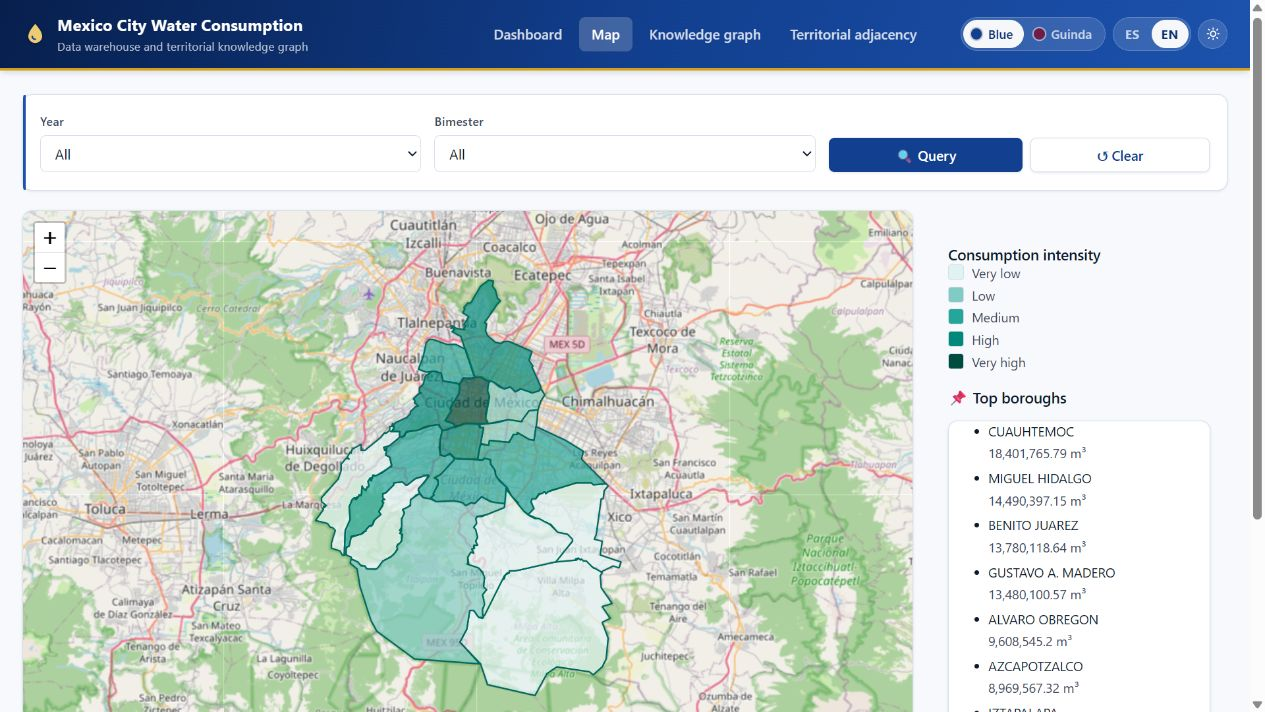
\includegraphics[width=\linewidth,keepaspectratio]{Mapa1.png}
  \caption{Choropleth retrieval by borough.\\
  \icokg{\scriptsize\url{https://gabrielhuav.github.io/Data_Warehouse_static/mapa.html}}}
  \label{fig:mapa-a}
\end{subfigure}\hfill
\begin{subfigure}[t]{0.485\textwidth}
  \centering
  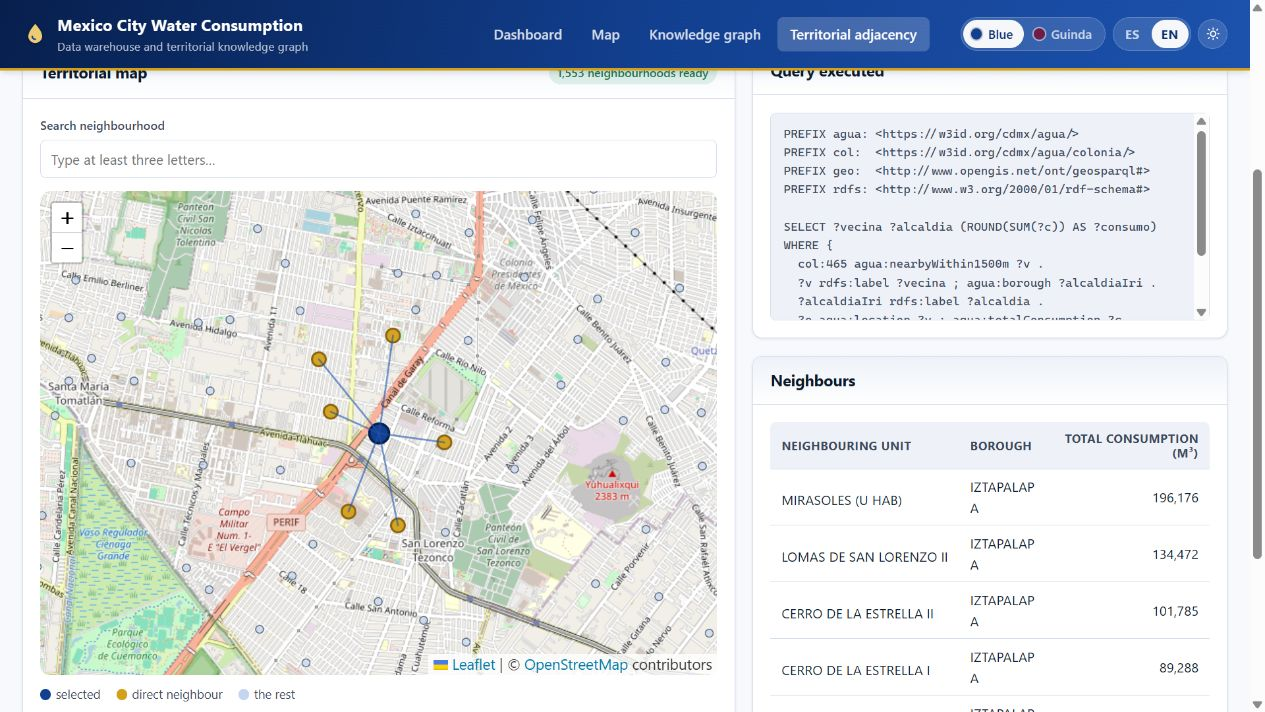
\includegraphics[width=\linewidth,keepaspectratio]{Mapa2.png}
  \caption{\icokg{Adjacency as graph traversal, with the \texttt{agua:nearbyWithin1500m}
  query and its result.\\
  \scriptsize\url{https://gabrielhuav.github.io/Data_Warehouse_static/vecindad.html?alcaldia=IZTAPALAPA&colonia=AO\%20DE\%20JUAREZ}}}
  \label{fig:mapa-b}
\end{subfigure}
\caption{\icokg{The two retrieval modes of the static demonstration, both
running in the browser without a server; each caption links to the exact view
captured. Base map \copyright{} OpenStreetMap contributors (ODbL).}}
\label{fig:mapa}
\end{figure}


\subsection{Implementation of the Atypical-Consumption Module}

The current version replaces supervised prediction with an exploratory detection
module oriented to analytical retrieval: because the open source carries no
anomaly labels, the system computes statistical indicators over the retrieved
records instead of training a model. \icokg{The procedure runs unsupervised on the
frontend. Consumption is aggregated by neighbourhood, each neighbourhood is
compared against the others of its own borough, and the units with the largest
deviation are ranked as candidates for inspection.} Flagging patterns that
require later review keeps the practical value of the component without
presenting a prediction as if it had been trained against ground truth.

Formally, each neighbourhood $g$ receives an atypicality score:
\begingroup
\setlength{\abovedisplayskip}{3pt}
\setlength{\belowdisplayskip}{3pt}
\setlength{\abovedisplayshortskip}{0pt}
\setlength{\belowdisplayshortskip}{3pt}
\begin{equation}
A_g = \left| \frac{x_g - \mu}{\sigma + \epsilon} \right|,
\end{equation}
\endgroup
where $x_g$ is the aggregate consumption of a neighbourhood, \icokg{$\mu$ and $\sigma$ are the mean and standard deviation of the neighbourhoods of its own borough ---the comparison set implemented in \texttt{assets/atipicos.js}---}, and $\epsilon$ prevents division by zero. The groups with the largest $A_g$ are reported in the interface as zones with atypical consumption.

\begin{icokgblock}
Two clarifications delimit the module. It is \emph{exploratory} and not a causal
predictor: a high $A_g$ states that a zone departs from its comparison set, not
why. And it does \emph{not} perform real-time leak detection, since no leak
reports, work orders or network telemetry are integrated into the warehouse and
the evaluation in Section~\ref{sec:res} rests exclusively on synthetically
injected perturbations. Its role is the ranking function of the retrieval
framework: the choropleth answers ``how much is consumed here'', the module
answers ``which units should I look at first'', which is the ordering problem at
the centre of information retrieval~\cite{purves2018}.
\end{icokgblock}

\begin{icokgblock}
\section{From the Dimensional Model to a Knowledge Graph}
\label{sec:kg}

\subsection{Rationale: Why a Star Schema, and What a Graph Adds}

The star schema was not chosen by default. The dominant workload is the repeated
aggregation of one numeric measure over three conformed dimensions with filters
chosen interactively, which is what dimensional modelling was designed
for~\cite{kimball}: constant join depth and aggregation by a single grouped scan.
A graph would pay a traversal cost for joins that foreign keys already resolve.
What a graph adds is complementary: \emph{interoperability}, since a standard
vocabulary makes the resource linkable to other municipal datasets without prior schema
agreement, the recurring obstacle in the open-data literature~\cite{vetro2016}; \emph{topological expressiveness}, since
questions such as ``which neighbourhoods adjacent to an atypical zone also exceed
the borough mean'' are natural traversals and awkward over a flat territorial
dimension; and \emph{entity reconciliation}, since \icokg{stable identifiers would resolve
the label heterogeneity our ETL absorbs through normalisation rules ---the
\texttt{w3id} namespace used here is not yet registered for dereferencing, which
we leave as future work}. We
therefore keep the star schema as the analytical store and derive the RDF layer
by a declarative mapping, so that neither representation is maintained by hand.

\subsection{Vocabulary Alignment and R2RML Mapping}

The correspondence between a star schema and the RDF Data Cube~\cite{datacube}
is close to mechanical, which is what makes this layer inexpensive to maintain: a
fact row becomes a \texttt{qb:Observation}, the measures become
\texttt{qb:MeasureProperty}, the time and location dimensions become
\texttt{qb:DimensionProperty}, the neighbourhood entity becomes a
\texttt{geo:Feature} with its \texttt{geo:asWKT} geometry, territorial adjacency
becomes \icokg{the project-defined \texttt{agua:nearbyWithin1500m}}, and the development index becomes a
\texttt{skos:Concept} \icokg{in a declared \texttt{skos:ConceptScheme} with an explicit numeric rank}. The mapping is expressed in R2RML~\cite{r2rml} and distributed with the archived
release, declaring seven triples maps over both fact tables, the territorial
dimension and its geometry, the derived adjacency, the temporal dimension and the
index scheme. \icokg{A companion \texttt{schema.ttl} supplies what the mapping alone
cannot: the \texttt{qb:DataStructureDefinition} for both cubes, its components
typed as dimension, measure or attribute, the cubic-metre unit and the ordinal
scale. Loaded together with the browser
graph, it satisfies the Data Cube integrity constraints IC-1, IC-2, IC-3 and
IC-11 with zero violations, reproducible with \texttt{scripts/validar\_datacube.py};
the check is stated for the published demonstration graph, not for the complete
materialisation. The alignment is therefore a validated property rather than a
nominal reuse of two terms.}
Materialising it yields \icokg{on the order of $7.6\times10^{5}$ triples} over
71{,}067 observations, 1{,}553 territorial features, 181 temporal entities and
the four index members.


Two properties of the geospatial layer bound what the traversal can claim. The
warehouse stores \emph{points}, not polygons: each neighbourhood is the centroid
of its readings, recovered from coordinates present in the source export but
dropped by the original loading schema. The substitution is defensible at
this scale ---the 22,930 distinct coordinates are never shared between two
neighbourhoods and the median neighbourhood diameter is 0.63~km--- though coarse
for the ten neighbourhoods above three kilometres. \icokg{Because centroids are points, no Simple Features boundary relation applies:
\texttt{geo:sfTouches} is undefined for point/point geometries, and relabelling a
distance threshold as a standardised topological predicate would misstate what
the data support. The mapping therefore declares its own
\texttt{agua:nearbyWithin1500m}, documented in \texttt{schema.ttl} as centroid
proximity below 1.5~km. Official polygons would allow \texttt{geo:sfTouches} in
the strict sense; that is a substitution in the source data, and we leave it as
future work.} \nuevo{Section~\ref{sec:kgmetro} takes that step for the metropolitan graph.}

\subsection{Territorial Retrieval as Graph Traversal}
\label{sec:sparql}

The value of the layer is that it makes a class of questions expressible that the
tabular interface does not naturally support. GeoSPARQL supplies the geometry
model~\cite{carhomburg2022}; \icokg{Listing~\ref{lst:sparql} is
the query the published interface executes verbatim}, retrieving the
neighbourhoods near a selected zone together with their own consumption, a
single traversal that the relational interface resolves only through an ad-hoc
spatial self-join, and which Fig.~\ref{fig:mapa-b} shows executing in the
published demonstration.

\begin{lstlisting}[caption={\icokg{Territorial traversal over the knowledge graph, as executed by \texttt{vecindad.html}.}},label={lst:sparql}]
PREFIX agua: <https://w3id.org/cdmx/agua/>
PREFIX col:  <https://w3id.org/cdmx/agua/colonia/>
PREFIX rdfs: <http://www.w3.org/2000/01/rdf-schema#>

SELECT ?vecina ?alcaldia (ROUND(SUM(?c)) AS ?consumo) WHERE {
  col:465 agua:nearbyWithin1500m ?v .
  ?v rdfs:label ?vecina ; agua:borough ?alcaldiaIri .
  ?alcaldiaIri rdfs:label ?alcaldia .
  ?o agua:location ?v ; agua:totalConsumption ?c .
} GROUP BY ?vecina ?alcaldia ORDER BY DESC(?consumo)
\end{lstlisting}

That the graph is queryable, and not merely declarable, is shown without any
server: the static deployment ships a browser-sized subset of \icokg{140,499} triples
with a SPARQL~1.1 engine \icokg{vendored in the release itself, so the
demonstration depends on no external service}. \icokg{The subset is an aggregate, not a slice: its observations live at the
neighbourhood-period grain in a separate \texttt{agua:aggobs/} namespace under
\texttt{agua:consumoCDMXDemo}, linked to the complete dataset through PROV-O.
Distinct identities avoid the contradictory RDF that reusing an IRI across grains
would produce if the graphs were merged; the price is that a query written
against the subset is not guaranteed to run unchanged against the full
materialisation.} The two
representations agree where they overlap: aggregating consumption by bimester
through SPARQL returns the same totals the reproduction script obtains in SQL.
\end{icokgblock}

\section{Results and Evaluation}
\label{sec:res}

\subsection{Integrated Data Volume}

The ETL process consolidated the water-consumption information of Mexico City into the dimensional warehouse. Table~\ref{tab:volumen_datos} presents the stored volume. \icokg{Each cardinality answers to a different grain and this must be read carefully. The 1,553 locations are the distinct borough--neighbourhood pairs and are coarser than the fact grain. The four index levels are the four members of the SACMEX ordinal scale, not three levels plus a residual. And the 181 time records are \emph{not} reading dates: they are the daily observations of the climate series integrated alongside the consumption data, from which the dimension is populated. The consumption source carries three reading dates only, one per bimester, so the fact table distributes its rows over those three while the climate facts use all 181. The shared temporal dimension at daily grain is what allows both to be queried together.}

\begin{table}[tbp]
\centering
\caption{Data volume stored in the data warehouse}
\label{tab:volumen_datos}
\begin{tabular}{lc}
\hline
\textbf{Table} & \textbf{Records} \\
\hline
\icokg{fact\_consumo\_agua} & 70,886 \\
\icokg{dim\_ubicacion} & 1,553 \\
\icokg{dim\_tiempo} & 181 \\
\icokg{dim\_indice\_des} & 4 \\
\hline
\end{tabular}
\end{table}

\subsection{Findings of the Consumption Analysis}

The analysis of the 70,886 consolidated records reveals the following consumption patterns in Mexico City:

\begin{itemize}
    \item \textbf{Territorial concentration:} The boroughs with the highest total consumption are Cuauht\'emoc and Miguel Hidalgo, followed by Benito Ju\'arez and Gustavo A. Madero (Table~\ref{tab:top5_alcaldias}).
    \item \textbf{Temporal distribution:} Consumption shows variations across the bimesters available in the warehouse. In the aggregated query by bimester, the highest total consumption was observed in bimester 2, followed by bimester 3 and bimester 1. Therefore, no direct causal relationship with dry or rainy periods is established without integrating additional climatic variables.
    \item \textbf{Relationship with the development index:} \nuevo{Neighbourhoods} with a High development index show a higher average consumption than those with a Low index, a descriptive association discussed in Section~\ref{sec:con}.
\end{itemize}

\begin{table}[tbp]
\centering
\caption{Five boroughs with the highest total water consumption}
\label{tab:top5_alcaldias}
\begin{tabular}{|l|r|}
\hline
\textbf{Borough} & \textbf{Total consumption} \\
\hline
Cuauht\'emoc & 18\,401\,765.79 \\
Miguel Hidalgo & 14\,490\,397.15 \\
Benito Ju\'arez & 13\,780\,118.64 \\
Gustavo A. Madero & 13\,480\,100.57 \\
\'Alvaro Obreg\'on & 9\,608\,545.20 \\
\hline
\end{tabular}
\end{table}



\begin{nuevobloque}
\subsection{Billed Volume and Consumption per Inhabitant}
\label{sec:percapita}

The conference version warned that totals are not a per-capita indicator
(Section~\ref{sec:disc}). Dividing the domestic billed volume of the semester by the
residents of private dwellings counted in the 2020 Census, the nearest count to
2019~\cite{inegi2021}, and by the semester's 181 days gives the figures of
Table~\ref{tab:percapita}. Two results follow. The first is that the ranking changes:
Benito Ju\'arez, third in total consumption, is first per inhabitant with 126.5
litres per day, while Gustavo A. Madero and Iztapalapa, fourth and seventh in
totals, fall to tenth and fourteenth. The second matters more. The city-wide
figure is 47.3 litres per inhabitant per day, or 53.9 including mixed-use billing,
about 38\,\% of the 123 litres per day that Medina-Rivas et al.~\cite{medina2022}
report for the same year from records provided by the utility. The gap does not
come from the export being incomplete. Annualised, its billed volume is about 243
million cubic metres, close to the 255 million that the utility reported as
billed in 2021 in answer to a public-information request~\cite{infocdmx2022}. It
is billing that captures only part of the water used: the export amounts to
7.7~m$^3$/s, about half of the 15.44~m$^3$/s of total consumption that Ramos-Bueno
et al.~\cite{ramosbueno2024} estimate for the city. The shortfall is concentrated
in the periphery, where 16.0 litres in Iztapalapa, 8.2 in Tl\'ahuac and 2.5 in
Milpa Alta cannot be the water people use. The clarifying note covers metered and
average billing only (Section~\ref{sec:grain}), so intakes billed without a volume
would leave no trace in the data; the Fiscal Code applies a fixed fee rather than
a volume to domestic intakes in colonias whose supply is officially classified as
by rota (\emph{tandeo}). That explanation
is plausible but cannot be confirmed from the export alone. Either way, the open
export is a faithful image of volumetric billing rather than of consumption, and
Table~\ref{tab:top5_alcaldias} ranks billing coverage as much as demand. This is
a question of validity rather than of completeness~\cite{vetro2016}: every record
may be present and the measure still answer a different question. The table is
reproducible with \texttt{scripts/per\_capita\_alcaldia.py}.

\begin{table}[tbp]
\centering
\caption{Domestic billed volume of the first semester of 2019 per resident of
private dwellings (2020 Census), by borough, with the change in rank from total
consumption (all uses) to consumption per inhabitant.}
\label{tab:percapita}
\begin{tabular}{lrrrc}
\hline
\textbf{Borough} & \textbf{Residents} & \textbf{Domestic (thousand m$^3$)} & \textbf{Litres per inhabitant per day} & \textbf{Rank: total to per inhabitant} \\
\hline
Benito Ju\'arez & 432,259 & 9,894.9 & 126.5 & 3 to 1 \\
Miguel Hidalgo & 412,529 & 8,640.5 & 115.7 & 2 to 2 \\
Cuauht\'emoc & 540,976 & 10,207.7 & 104.2 & 1 to 3 \\
Azcapotzalco & 431,347 & 6,153.8 & 78.8 & 6 to 4 \\
Iztacalco & 403,805 & 4,663.5 & 63.8 & 10 to 5 \\
Venustiano Carranza & 443,120 & 5,007.0 & 62.4 & 9 to 6 \\
Cuajimalpa de Morelos & 217,606 & 2,064.3 & 52.4 & 12 to 7 \\
\'Alvaro Obreg\'on & 757,117 & 6,590.2 & 48.1 & 5 to 8 \\
Coyoac\'an & 612,130 & 5,128.3 & 46.3 & 8 to 9 \\
Gustavo A. Madero & 1,162,914 & 9,196.4 & 43.7 & 4 to 10 \\
Tlalpan & 695,308 & 2,843.1 & 22.6 & 11 to 11 \\
La Magdalena Contreras & 246,785 & 845.0 & 18.9 & 14 to 12 \\
Xochimilco & 438,038 & 1,304.1 & 16.4 & 13 to 13 \\
Iztapalapa & 1,820,809 & 5,263.0 & 16.0 & 7 to 14 \\
Tl\'ahuac & 391,967 & 583.0 & 8.2 & 15 to 15 \\
Milpa Alta & 152,682 & 69.1 & 2.5 & 16 to 16 \\
\hline
\textbf{Mexico City} & \textbf{9,159,392} & \textbf{78,453.9} & \textbf{47.3} & \\
\hline
\end{tabular}
\end{table}
\end{nuevobloque}

\subsection{Quantitative Evaluation of the Atypical-Consumption Module}

With no anomaly labels in the open source, the module is evaluated against
injected ground truth. \icokg{The protocol scores \emph{the deployed
function itself}, not a proxy: consumption is aggregated by neighbourhood, $\mu$
and $\sigma$ are computed over the neighbourhoods of each borough, and $A_g$
ranks them, which is exactly what \texttt{assets/atipicos.js} computes. The
synthetic set reproduces the structure of the warehouse ---1,553
borough--neighbourhood pairs over three bimesters--- with 47 injected anomalies
per run, and the experiment is repeated over 20 seeds. The three detectors are
compared at equalised operating points, each emitting as many alerts as there are
injected anomalies, so precision, recall and F1 coincide by construction and the
areas under the curves characterise the ranking independently of any threshold
(Table~\ref{tab:eval_ml}).}

\begin{table}[tbp]
\centering
\caption{\icokg{Detection of injected anomalies, mean $\pm$ standard deviation over 20 seeds at equalised operating points. Reproducible with \texttt{evaluacion-ml/eval\_anomalias.py}, a script reconstructed for this artefact.}}
\label{tab:eval_ml}
\begin{tabular}{@{}lccc@{}}
\hline
\textbf{Method} & \textbf{P\,=\,R\,=\,F1} & \textbf{ROC-AUC} & \textbf{PR-AUC} \\
\hline
$A_g$ (deployed) & $0.581\pm0.040$ & $0.966\pm0.013$ & $0.677\pm0.047$ \\
Isolation Forest & $0.650\pm0.053$ & $0.971\pm0.013$ & $0.728\pm0.058$ \\
LOF & $0.493\pm0.075$ & $0.846\pm0.036$ & $0.464\pm0.075$ \\
\hline
\end{tabular}
\end{table}

\icokg{The deployed statistic is competitive with the strongest baseline: its
ROC-AUC of 0.966 lies within one standard deviation of the 0.971 of Isolation
Forest\nuevo{~\cite{liu2008}}, and it recovers 58\,\% of the injected anomalies against 65\,\%. That
0.069 difference is modest relative to the combined between-seed variability,
although Isolation Forest remains consistently superior at the evaluated
operating point. LOF\nuevo{~\cite{breunig2000}} is clearly worse (0.846), since
it looks for locally sparse neighbourhoods whereas the injected perturbations are
departures in global magnitude. An interpretable borough-relative z-score therefore
loses little ranking quality against an ensemble method a municipal analyst could
not inspect, which supports $A_g$ as a conservative exploratory filter, one that ranks a short list a utility can afford to inspect, and point to Isolation Forest as the natural improvement.}

\icokg{Two limitations remain. The perturbations are synthetic and their magnitude
is chosen, so the figures measure sensitivity to known deviations rather than
field performance against real leaks, for which the system is not designed and no
labelled data exist. And the comparison rests on a single injection model; a
different anomaly shape could reorder the methods.}

\begin{nuevobloque}
\subsection{Sensitivity of the Detection Module}
\label{sec:sens}

The second limitation can be removed experimentally. The protocol was repeated
varying one factor of the injection model at a time: the prevalence (1, 3, 5 and
10\,\%), the share of spikes among the anomalies (10 to 90\,\%) and their
magnitude, from subtle (spikes $\times$1.5--2, drops $\times$0.50--0.67) through
moderate ($\times$2--3 and $\times$0.33--0.50) to the strong setting of
Table~\ref{tab:eval_ml} ($\times$3--6 and $\times$0.05--0.25). Each of the twelve
settings ran over the same 20 seeds, 240 runs in all, with the same territorial
identities, deployed function, baselines and equalised operating point; recall
is additionally reported separately for spikes and for drops. With the published
setting the script reproduces Table~\ref{tab:eval_ml} exactly, and it adds a
fourth detector, log-$A_g$: the same statistic computed on the logarithm of the
aggregate consumption. Because anomalies are at most a tenth of the units, the
area under the precision--recall curve is the more informative summary of a
ranking~\cite{saito2015}. Everything is reproducible with
\texttt{evaluacion-ml/sensibilidad\_anomalias.py}.

The deployed statistic turns out to be structurally blind to drops
(Fig.~\ref{fig:sens}a). Under the published setting it finds 82\,\% of the
injected spikes and 2\,\% of the drops. The cause is arithmetic, not
statistical. A drop can lower a neighbourhood's consumption by at most its whole
value, so a neighbourhood below its borough mean scores at most
$\mu/\sigma$, the inverse of the borough's coefficient of variation, whereas a
spike's score is unbounded. With the dispersion of the synthetic boroughs that
ceiling is about 2.3, below the scores that ordinary neighbourhoods in the right
tail already reach, so when the alert budget is spent on the largest scores the
drops are never reached. The published precision of 0.58 is therefore the share
of spikes found weighted by the share of spikes injected, and it falls to 0.12
when nine anomalies in ten are drops (Fig.~\ref{fig:sens}b and
Table~\ref{tab:sens}).

On a logarithmic scale a multiplicative drop and a multiplicative spike lie at
symmetric distances from the mean, and log-$A_g$ removes the blindness: under
the published setting it finds 71\,\% of spikes and 92\,\% of drops, raising
precision from 0.581 to 0.770 and the area under the precision--recall curve from
0.677 to 0.860, above Isolation Forest (0.650 and 0.728). The advantage holds
across prevalences and compositions (Table~\ref{tab:sens}) and fades as the
anomalies weaken: at moderate magnitude it only ties Isolation Forest (0.398), and
at subtle magnitude every detector stays below 0.20, where the limit is the
magnitude of the departure rather than the scale of the score. The comparison is
not neutral, however: the synthetic consumption is log-normal by construction,
which makes log-$A_g$ the matched statistic, so its synthetic margin is an upper
bound. Section~\ref{sec:real} confronts both scores with the real distribution.

\begin{figure}[tbp]
\centering
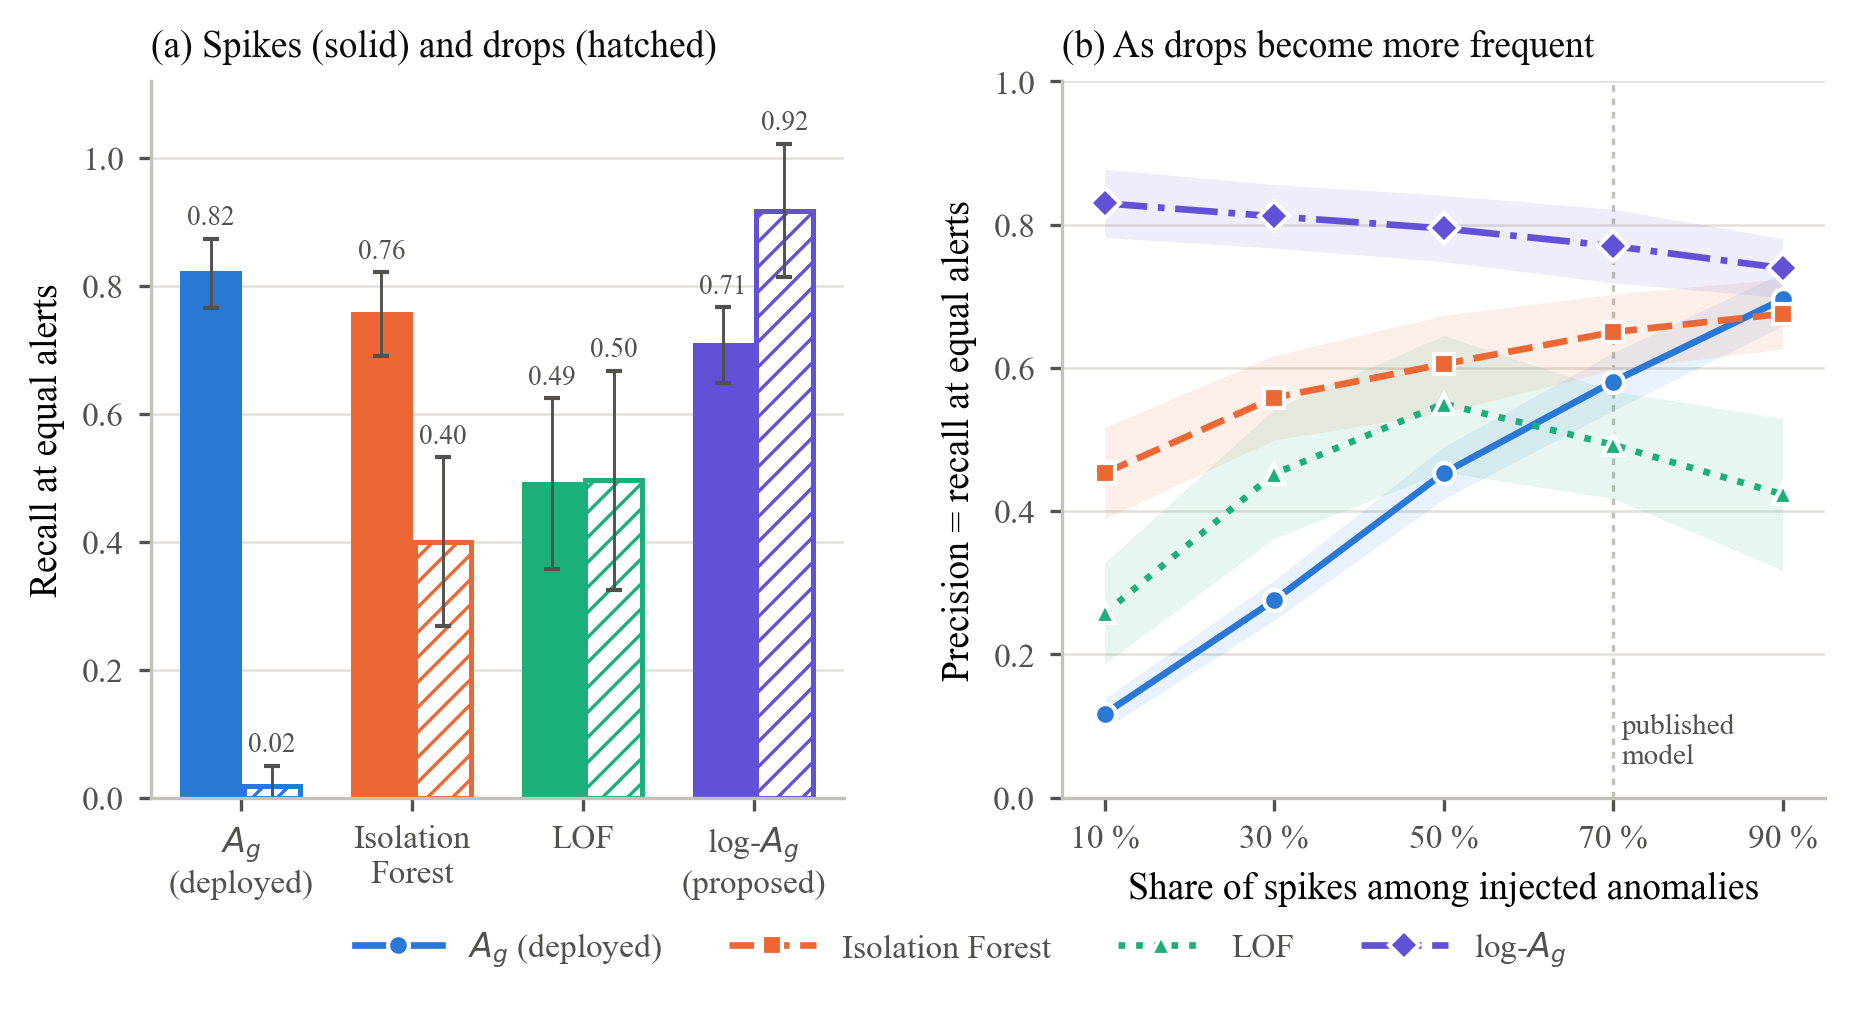
\includegraphics[width=\textwidth]{figura_anomalias.png}
\caption{Recall on injected spikes and drops under the published setting (a),
and precision at the equalised operating point as the share of spikes varies (b).
Mean over 20 seeds; bars and bands show one standard deviation.}
\label{fig:sens}
\end{figure}

\begin{table}[tbp]
\centering
\caption{Precision at the equalised operating point (equal to recall and F1) under
each injection setting, mean over 20 seeds; standard deviations stay between 0.015
and 0.124. Published setting: 3\,\% prevalence, 70\,\% spikes, strong magnitude.}
\label{tab:sens}
\begin{tabular}{lcccc}
\hline
\textbf{Setting} & \textbf{$A_g$} & \textbf{Isolation Forest} & \textbf{LOF} & \textbf{log-$A_g$} \\
\hline
Published setting & 0.581 & 0.650 & 0.493 & 0.770 \\
Prevalence 1\,\% & 0.491 & 0.544 & 0.600 & 0.709 \\
Prevalence 10\,\% & 0.749 & 0.763 & 0.303 & 0.834 \\
10\,\% spikes, 90\,\% drops & 0.117 & 0.453 & 0.257 & 0.830 \\
50\,\% spikes, 50\,\% drops & 0.453 & 0.605 & 0.550 & 0.795 \\
90\,\% spikes, 10\,\% drops & 0.696 & 0.676 & 0.423 & 0.739 \\
Moderate magnitude & 0.365 & 0.398 & 0.304 & 0.398 \\
Subtle magnitude & 0.181 & 0.183 & 0.122 & 0.173 \\
\hline
\end{tabular}
\end{table}

\subsection{The Deployed Ranking on the Real Data}
\label{sec:real}

The arithmetic bound does not depend on the synthetic generator, so it can be
checked on the warehouse itself. Replicating the deployed computation over the
1,553 borough--neighbourhood totals of the published export, with no filter,
shows totals that are strongly right-skewed within every borough but one (median
skewness 1.98) and much less skewed in logarithms (median $-$0.76). The ceiling
$\mu/\sigma$ for a neighbourhood below its borough mean has a median of 0.85
across boroughs (0.27 to 1.64), and the highest score any of the 1,022
below-mean neighbourhoods actually reaches is 1.46, whereas the fifteenth entry
the interface lists scores 3.85. Not one of the 15 neighbourhoods the module
shows, nor of the top 3\,\% (47), lies below its borough mean: as deployed, the
module can only ever report excess consumption.

The log-scale score does not settle the matter on real data; it inverts it.
Because log totals are left-skewed, their long tail is the low one, and all 15
neighbourhoods at the top of the log-$A_g$ ranking, and 45 of the top 47, lie
below their borough mean; the two top-15 lists share no neighbourhood. A further
29 neighbourhoods have no billed volume at all over the semester, 27 of them with
records in all three bimesters, concentrated in Tlalpan (12), Iztapalapa (6) and
La Magdalena Contreras (5). Neither score treats them sensibly: $A_g$ ranks them
low and their logarithm is undefined. On these data no single symmetric score
serves both directions. The design the evidence supports is three lists: excess
and deficit, each ranked by log-$A_g$ within its own direction, and
neighbourhoods without billed volume as a separate flag, which in a source that
bills unmetered intakes by averages (Section~\ref{sec:grain}) may signal a data
gap as much as an absence of use, which is why earlier spatial studies exclude
colonias with zero consumption or no metering~\cite{ramosbueno2021}. The analysis is reproducible with
\texttt{evaluacion-ml/ranking\_real.py}.

\subsection{From the City to the Metropolitan Area}
\label{sec:metro}

The open export stops at the city boundary, but the water system does not. We therefore extended
the warehouse additively to the official metropolitan delimitation of 2020~\cite{conapo2025b}: 63
municipalities, of which 16 are boroughs, 45 lie in the State of Mexico and two in Hidalgo. Sixty-two
files, each checked against a manifest of sizes and hashes before loading, now feed 2.79 million
rows in 45 tables, joined to the original location dimension through a conformed municipal
dimension; the original fact tables are untouched. The new facts cover municipal services and
billing~\cite{inegicngmd}, water revenue~\cite{shcp2026}, aquifers and wells~\cite{conagua2026a},
dams~\cite{conagua2026b}, drought~\cite{smn2026}, water quality~\cite{conaguacalidad},
marginalisation~\cite{conapo2025a}, land motion~\cite{khorrami2023} and 555,752 citizen
reports~\cite{sacmexreportes}.

Integration exposes what no single source shows. Municipal volumes cannot be compared without a
filter: of the 47 municipalities outside Mexico City, 24 report no volume, 7 fall outside a
plausibility band of 10 to 400 litres per inhabitant per day and 16 remain
(Fig.~\ref{fig:zm-a}), while the revenue they declare does track federal records (Spearman 0.934
over 89 municipalities of the State of Mexico, Pearson 0.322), which confines the errors to a
few captures. The reports also bound what can be asked of 2019: the source records no leaks before
2021, so all 39,685 reports of the semester are water shortages. Across 1,508 neighbourhoods, billed
volume barely ranks shortage reports (Spearman 0.18), and the 435 neighbourhoods billed below 10
litres file almost as many reports per thousand inhabitants as the rest (4.15 against 4.93).
Near-zero billing therefore does not mean near-zero demand, which supports the reading of
Section~\ref{sec:percapita}. So does access: about 238,000 people in the metropolitan area live in
dwellings without piped water, and in Mexico City the five boroughs with the
largest share of them are among the six with the lowest billed volume. Groundwater gives the
physical context. The four aquifers beneath the urban area extract between 1.49 and 1.96 times
their recharge, and in wells read in both years the mean water table fell between 6.0 and 18.7
metres from 2010 to 2019.

\begin{figure}[tbp]
\centering
\begin{subfigure}[t]{0.485\textwidth}
  \centering
  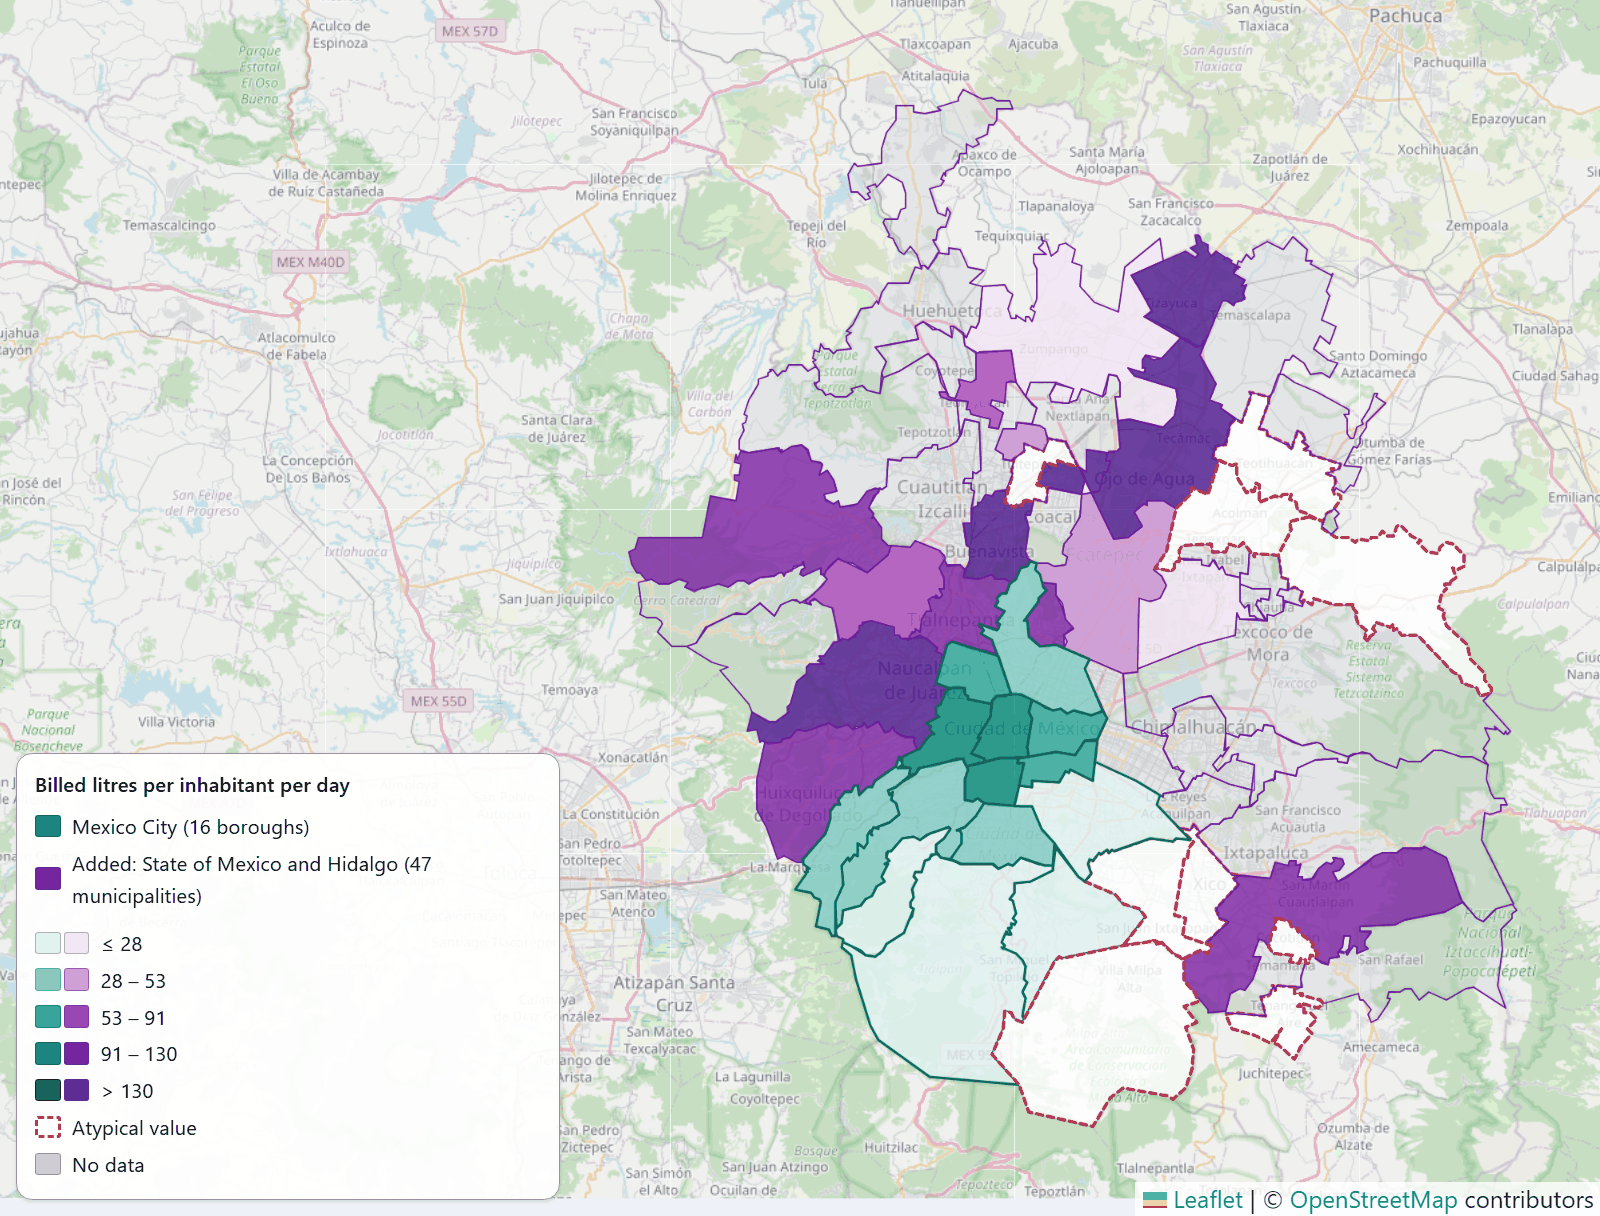
\includegraphics[width=\linewidth,keepaspectratio]{figura_zm_volumen.png}
  \caption{Billed litres per inhabitant per day.}
  \label{fig:zm-a}
\end{subfigure}\hfill
\begin{subfigure}[t]{0.485\textwidth}
  \centering
  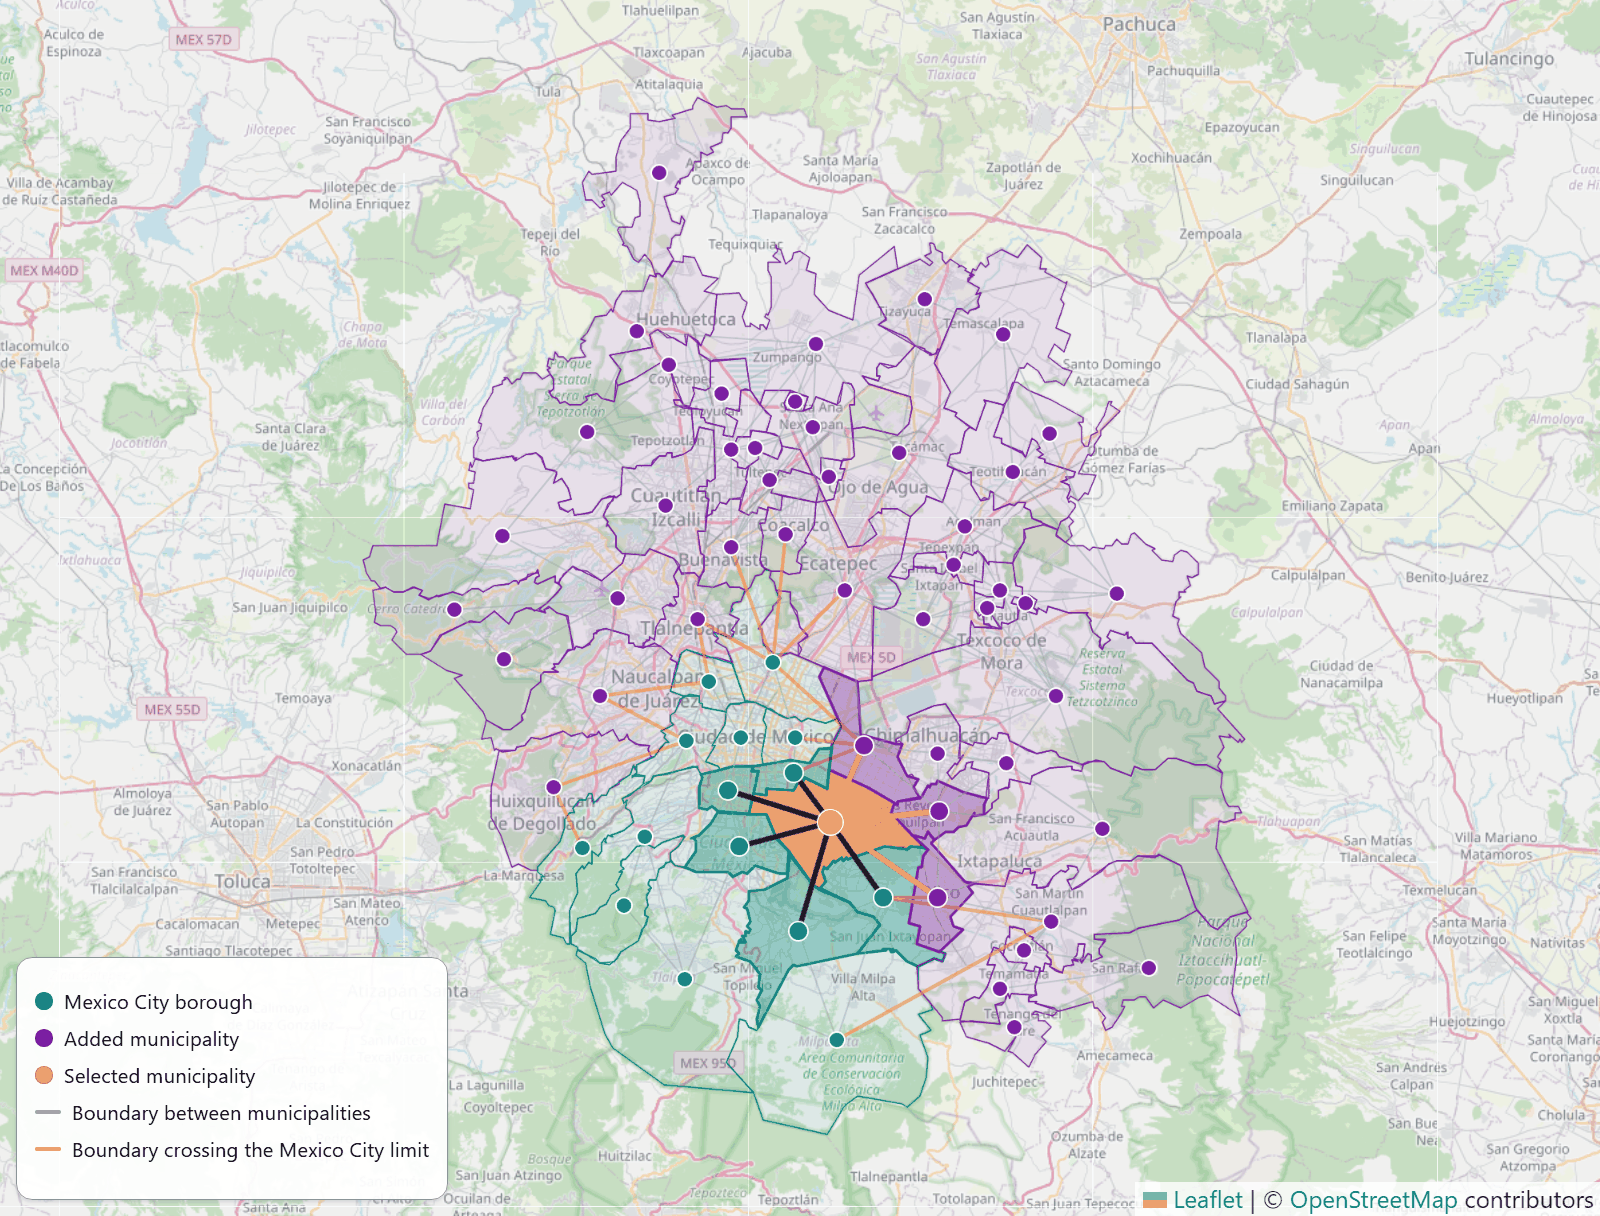
\includegraphics[width=\linewidth,keepaspectratio]{figura_zm_grafo.png}
  \caption{The graph: municipalities and shared boundaries.}
  \label{fig:zm-b}
\end{subfigure}
\caption{The metropolitan map and graph: Mexico City in green, the added municipalities in purple. In (a), stronger colour marks a higher available value, not higher use; in (b), orange edges cross the city limit. Base map \copyright{} OpenStreetMap contributors (ODbL).}
\label{fig:zm}
\end{figure}

The static deployment follows the warehouse without a server. Each layer of the map
(\url{https://gabrielhuav.github.io/Data_Warehouse_ZMVM/ijcopi/mapa-zm.html}) is the literal
result of one of fifteen SQL queries distributed in the repository, exported to \texttt{JSON} with
its hash, and \texttt{verificar\_mapa.py} repeats every query and compares the result byte by byte
with the published files. A warehouse rebuilt from a clean clone returned the same bytes for all
fifteen queries.

\subsection{A Metropolitan Knowledge Graph}
\label{sec:kgmetro}

The graph of Section~\ref{sec:kg} stops at the city boundary and joins neighbourhoods by centroid
proximity, because the warehouse held only points. Official polygons lift both limits. A second
R2RML mapping materialises the extended warehouse into 82,393 triples, linked to the boroughs and
neighbourhoods of the first graph so that the two can be merged. Its 5,830 neighbourhoods carry
15,510 pairs of strict \texttt{geo:sfTouches}. Municipalities required more care: the official
polygons overlap by up to 0.49~m$^2$, so the strict relation fails for pairs that do adjoin, and
rather than misuse the standard predicate the graph declares \texttt{agua:sharesBoundaryWith} for
the 163 pairs sharing at least 50~m of boundary (Fig.~\ref{fig:zm-b}). A value the sources do not
report produces no triple, so absence stays explicit. Traversal then crosses what the sources keep
apart: 18 municipal boundaries and 169 neighbourhood adjacencies cross the Mexico City limit;
subsidence does not stop there, with Nezahualc\'oyotl sinking 23.5~cm per year next to Venustiano
Carranza at 16.5~cm; and 21 municipalities that report no volume overlie an aquifer extracting more
than 1.5 times its recharge, context the billing data cannot give. Every relation matches its
warehouse table, and the example queries run in the browser against the published graph
(\url{https://gabrielhuav.github.io/Data_Warehouse_ZMVM/ijcopi/grafo-zm.html}).
\end{nuevobloque}

\subsection{Performance Metrics}

\icokg{Lighthouse~13.4.1, run against the permanent static deployment, scores 89
on emulated desktop (first contentful paint 0.2~s, largest 0.3~s, total blocking
time 200~ms) and 76 on emulated mobile over throttled 4G; accessibility, best
practices and SEO score 100 on both. The remaining bound is structural: the
static version downloads the full 3.9~MB export and aggregates on the client, so
what a server computes once is computed by each visitor.}


\subsubsection*{Query Performance over the Total Data Volume.}

\begin{icokgblock}
Frontend metrics do not characterise the retrieval layer, so four analytical
workloads were timed directly against the warehouse over all 70,886 fact rows: a
paginated retrieval, a full-scan aggregation by borough, a full-scan aggregation
by neighbourhood and bimester ---the heaviest query the dashboard issues--- and a
top-$N$ ranking. Each ran 200 times after ten warm-up calls on twelve logical cores with 32~GB of
RAM and PostgreSQL~16.14 in a container, which is what makes the reported
percentile meaningful. These are SQL latencies measured at
the database, excluding serialisation and transport.

The profile, reported in Table~\ref{tab:api_perf}, is the expected one for a
star schema of this size: the three
workloads that resolve through the dimensions stay near 25~ms while scanning the
full fact table, whereas the aggregation by neighbourhood and bimester costs four
times more because it groups over 1,553 locations rather than sixteen. The
heaviest interactive query returns in about a tenth of a second, and the gap
between mean and p95 stays below 25\,\% throughout, indicating that the cost is
dominated by the scan rather than by contention.

\begin{table}[tbp]
\centering
\caption{Response time of the retrieval workloads over the complete warehouse
(70,886 fact rows), 200 executions after ten warm-up calls.}
\label{tab:api_perf}
\footnotesize
\begin{tabularx}{\textwidth}{@{}Yrrr@{}}
\hline
\textbf{Workload} & \textbf{Mean (ms)} & \textbf{p95 (ms)} & \textbf{Executions} \\
\hline
Paginated retrieval (\texttt{limit=100})   &  32.3 &  35.2 & 200 \\
Full aggregation by borough                &  24.1 &  27.0 & 200 \\
Aggregation by neighbourhood and bimester  & 101.3 & 125.4 & 200 \\
Top-10 neighbourhoods with ordering        &  23.1 &  23.6 & 200 \\
\hline
\end{tabularx}
\end{table}
\end{icokgblock}

\subsection{Functional Tests}

\icokg{The operation of the ETL processes, the persistence in PostgreSQL, the parameterized queries and the information retrieval was verified.} The tests included queries parameterized by year, bimester, borough, and \nuevo{neighbourhood}; aggregated retrieval (total and average consumption by \nuevo{neighbourhood}); generation of JSON responses; geospatial retrieval for visualization; and pagination with configurable limits. All modules produced results consistent with the expected structure. The dimensional model thus retrieves territorial information through combined filters of time, location and development index over the 70,886 records, supporting consumption queries by \nuevo{neighbourhood} and borough, temporal aggregation, coordinate retrieval, geospatial exploration and ordering by total consumption.

\begin{icokgblock}
\section{Discussion}
\label{sec:disc}

Against the closest antecedents the contribution is one of \emph{provenance and
preservation} rather than of scale. Soares et al.~\cite{soares2019} and Abecker
et al.~\cite{abecker2014} begin from data an organisation already controls; this
work begins from a public export with no schema, versioning or update cadence,
which moves the difficulty from modelling to consolidation and is why the
cleaning criteria and their yield are reported explicitly. The second difference
is durability: those systems depend on a running service, whereas here interface,
graph and data are preserved as static artefacts any reader can
re-execute~\cite{sandve2013,hill2023}.

The practical implication is a caution about how the totals should be read. The
boroughs that consume most are not those that consume most per inhabitant:
Cuauht\'emoc and Miguel Hidalgo concentrate commercial activity, and the
warehouse supports the distinction because the source separates domestic from
non-domestic billing ---the non-domestic share reaches 32.5\,\% in Cuauht\'emoc
against 20.3\,\% in Gustavo A. Madero, twelve points apart between boroughs whose
totals differ by barely a third. Total consumption is therefore not a per-capita
indicator and should not be used as one for allocating supply interventions; the
per-account average, also stored, is the appropriate measure. \nuevo{The
per-inhabitant figures of Section~\ref{sec:percapita} confirm the reordering.}
\end{icokgblock}

\section{Conclusions and Future Work}
\label{sec:con}

\subsection{Conclusions}

A data warehouse was presented for the territorial information retrieval of water consumption in Mexico City, built from open sources through a reproducible ETL process and published with a continuous-deployment methodology that guarantees a permanent functional demonstration. The solution consolidated 70,886 consumption records and 1,553 locations across the 16 boroughs into a dimensional star schema on PostgreSQL.

The findings reveal that water consumption in Mexico City is concentrated in the boroughs of Cuauht\'emoc and Miguel Hidalgo (Table~\ref{tab:top5_alcaldias})\nuevo{ in billed totals, although Benito Ju\'arez leads per inhabitant and volumetric billing captures little of the consumption of the eastern and southern periphery (Table~\ref{tab:percapita})}, and that it varies across the available bimesters without establishing in this work a causal relationship with dry or rainy periods.

\icokg{The three central contributions ---the consolidation ETL, the validated graph layer derived from it, and the always-accessible demo methodology--- constitute} a replicable method for bringing heterogeneous official open data to queryable and verifiable territorial information. \nuevo{The extension adds a negative result: as deployed, the atypical-consumption module can only report excess consumption, and on the real data a log-scale score must be presented as separate lists for excess and deficit. Extending the warehouse to the 63 municipalities of the metropolitan area shows that municipal volumes need a quality filter before any comparison, and that low billing cannot be read as low demand.}

\begin{icokgblock}
\subsection{Threats to Validity and Limitations}

\nuevo{Six} limitations bound what may be concluded. The temporal extent is the first:
the source publishes three bimesters of a single year, so the seasonal variation
observed is a within-semester comparison and the climate correlation rests on
three aggregated points, enough to describe a direction but not to estimate one.
The second concerns the anomaly module, whose evaluation uses synthetic
perturbations aligned with the detectors; its figures are an upper bound and say
nothing about real leaks. \nuevo{The sensitivity analysis widens the injection model
but not its log-normal family.} The third is geometric: neighbourhoods are represented
by centroids rather than polygons, so the adjacency projected as
\icokg{\texttt{agua:nearbyWithin1500m}} is proximity within 1.5~km and not shared boundaries. The
fourth is descriptive: the association between development index and consumption
is an observation over the warehouse, and attributing it to a socioeconomic
mechanism would require an external source the warehouse does not
integrate. \nuevo{The fifth is the billing basis and its coverage: values mix
metered and averaged billing in an undisclosed proportion and add up to about
38\,\% of published per-capita consumption, with the gap concentrated in the
periphery. Territorial contrasts and atypicality scores therefore describe billing,
and match physical use only where intakes are metered. The sixth concerns the metropolitan layers: they combine reference years from 2018 to 2020,
the neighbourhood polygons are CONAPO's rather than the utility's, several joins rest on spatial
proximity, and reports count what citizens file, not what is missing.}

\subsection{Future Work}

The most immediate line is to materialise the knowledge graph into a persistent
triple store with a public SPARQL endpoint, and to replace the centroid-based
adjacency with official neighbourhood polygons, which would make the topological
predicates exact\nuevo{; the metropolitan graph already does so with CONAPO's polygons}. Aligning the territorial identifiers with external authorities
would let the resource be joined with other municipal datasets without prior
schema agreement, which is the interoperability argument that motivates the graph
layer. The anomaly module should be re-evaluated when labelled leak data exist\nuevo{,
with the three-list design of Section~\ref{sec:real} implemented in the interface}.
\nuevo{A data cube over the extended warehouse is the next step for the metropolitan analysis.}
Finally, the method transfers to other open urban-data domains ---mobility, air
quality and seismic risk--- where the same combination of dispersed official
files and absent query tooling recurs.
\end{icokgblock}

\begin{icokgblock}
\section*{Declaration on the Use of Generative AI}

The authors used a generative AI assistant, under their direction, for language
editing, drafting text subsequently revised and approved by
the authors, \nuevo{locating data sources,} and writing the \nuevo{scripts, queries, map and graph mapping} distributed with the artefact. The
research questions and the interpretation of the results are the authors' own work.
The authors take full responsibility for the
content.
\end{icokgblock}

\section*{Disclosure of Interests}
The authors declare that they have no conflicts of interest relevant to the content of this article.

% [Author Contributions: omitted for double-blind review; to be restored in the camera-ready version.]
% [Acknowledgments: omitted for double-blind review; to be restored in the camera-ready version.]

\begingroup\footnotesize\setlength{\parskip}{0pt}
\begin{thebibliography}{99}
\bibitem{abecker2014} Abecker, A., Brauer, T., Magoutas, B., Mentzas, G., Papageorgiou, N., Quenzer, M.: A Sensor and Semantic Data Warehouse for Integrated Water Resource Management. EnviroInfo 2014. BIS-Verlag, Oldenburg (2014)

\bibitem{berro2015} Berro, A., Megdiche, I., Teste, O.: A Content-Driven ETL Processes for Open Data. In: Bassiliades, N., et al. (eds.) New Trends in Database and Information Systems II. Springer, Cham (2015). \url{https://doi.org/10.1007/978-3-319-10518-5_3}

\bibitem{carhomburg2022}\icokg{ Car, N.J., Homburg, T.: GeoSPARQL 1.1: motivations, details and applications of the decadal update to the most important geospatial LOD standard. ISPRS International Journal of Geo-Information \textbf{11}(2), 117 (2022). \url{https://doi.org/10.3390/ijgi11020117}}

\bibitem{hill2023} Hill, D., Dunham, C., Larsen, D.A., Collins, M.: Operationalizing an open-source dashboard for wastewater-based surveillance. MethodsX \textbf{11}, 102299 (2023). \url{https://doi.org/10.1016/j.mex.2023.102299}

\bibitem{kimball} Kimball, R., Ross, M.: The Data Warehouse Toolkit: The Definitive Guide to Dimensional Modeling. 3rd edn. Wiley, Indianapolis (2013). ISBN 9781118530801

\bibitem{purves2018} Purves, R.S., Clough, P., Jones, C.B., Hall, M.H., Murdock, V.: Geographic Information Retrieval. Foundations and Trends in Information Retrieval \textbf{12}(2--3), 164--318 (2018). \url{https://doi.org/10.1561/1500000034}

\bibitem{roussey2023}\icokg{ Roussey, C., Gu\'eret, C., Laporte, M.-A.: Editorial: knowledge graph technologies --- the next frontier of the food, agriculture, and water domains. Frontiers in Artificial Intelligence \textbf{6}, 1319844 (2023). \url{https://doi.org/10.3389/frai.2023.1319844}}

\bibitem{sacmex2026} SACMEX: Consumo de agua. Resource \emph{Consumo Agua (1\textsuperscript{o} Semestre 2019)}, CSV, with data dictionary and clarifying note. Portal de Datos Abiertos de la Ciudad de M\'exico, Agencia Digital de Innovaci\'on P\'ublica. Resource migrated 28 August 2026. \url{https://datos.cdmx.gob.mx/dataset/consumo-agua}. Accessed 18 October 2026

\bibitem{velazquez2026icokg} Vel\'azquez Arrieta, E.U., Pulido Morales, O.F., Garc\'ia L\'opez, E., Hern\'andez Mart\'inez, C.A., Hurtado Avil\'es, G.: Territorial Information Retrieval from Heterogeneous Open Data through the Construction of a Data Warehouse for Water Management in Mexico City. In: Proceedings of ICOKG 2026. Springer (in press)

\bibitem{medina2022} Medina-Rivas, C.M., Rodr\'iguez-Tapia, L., Morales-Novelo, J.A., Revollo-Fern\'andez, D.A.: Spatial inequality of domestic water consumption in Mexico city. Water Resources and Economics \textbf{40}, 100210 (2022). \url{https://doi.org/10.1016/j.wre.2022.100210}

\bibitem{medina2025} Medina-Rivas, C.M., Morales-Novelo, J.A., Rodr\'iguez-Tapia, L., Revollo-Fern\'andez, D.A.: Mexico city's decline in per capita domestic water use: a comprehensive spatial-temporal study. Urban Water Journal \textbf{22}(1), 1--15 (2025). \url{https://doi.org/10.1080/1573062X.2024.2423400}

\bibitem{ramosbueno2021} Ramos-Bueno, A., Perevochtchikova, M., Chang, H.: Socio-spatial analysis of residential water demand in Mexico City. Tecnolog\'ia y Ciencias del Agua \textbf{12}(2), 59--110 (2021). \url{https://doi.org/10.24850/j-tyca-2021-02-02}

\bibitem{ramosbueno2024} Ramos-Bueno, A., Galeana-Pizaña, J.M., Perevochtchikova, M.: Urban water consumption analysis through a spatial panel modeling approach: a case study of Mexico City, 2004--2022. Water Supply \textbf{24}(9), 3179--3195 (2024). \url{https://doi.org/10.2166/ws.2024.191}

\bibitem{hernandez2026} Hern\'andez-V\'azquez, I., Luna-S\'anchez, A.J., Hurtado-Perez, A.B., Claramunt, C., Zagal-Flores, R., Mata, F.: Analyzing Water Consumption Patterns in Mexico City: A GIS and Data Science Approach. In: Mata-Rivera, M.F., Zagal-Flores, R., Siabato, W. (eds.) Web and Wireless Geographical Information Systems. W2GIS 2025. LNCS, vol. 15946, pp. 123--137. Springer, Cham (2026). \url{https://doi.org/10.1007/978-3-032-01723-9_9}

\bibitem{daowz2027} Daowz Laguna, E.E., Mata-Rivera, M.F., Zagal, R., Claramunt, C., Hern\'andez-Nava, C.: Enhancing Spatio-Temporal Analysis of Urban Water Leak Reports Through LLM-Based Semantic Enrichment and Open Data: A Case Study of Mexico City. In: Peng, P., Jin, M. (eds.) Web and Wireless Geographical Information Systems. W2GIS 2026. LNCS, vol. 17231, pp. 62--76. Springer, Cham (2027). \url{https://doi.org/10.1007/978-3-032-42081-7_6}

\bibitem{lippolis2025} Lippolis, A.S., Lodi, G., Nuzzolese, A.G.: The Water Health Open Knowledge Graph. Scientific Data \textbf{12}, 274 (2025). \url{https://doi.org/10.1038/s41597-025-04537-4}

\bibitem{inegi2021} Instituto Nacional de Estad\'istica y Geograf\'ia: Censo de Poblaci\'on y Vivienda 2020. Principales resultados por localidad (ITER), Ciudad de M\'exico. INEGI (2021). \url{https://www.inegi.org.mx/programas/ccpv/2020/}

\bibitem{infocdmx2022} Instituto de Transparencia, Acceso a la Informaci\'on P\'ublica, Protecci\'on de Datos Personales y Rendici\'on de Cuentas de la Ciudad de M\'exico: Resoluci\'on del recurso de revisi\'on INFOCDMX/RR.IP.0679/2022 (sujeto obligado: Sistema de Aguas de la Ciudad de M\'exico) (2022). \url{https://documentosobligaciones.infocdmx.org.mx/ST/LTAIPRC-2016-OT/Art133/Fr01/2022/T02-INFOCDMX.RR.IP.0679.2022.pdf}

\bibitem{liu2008} Liu, F.T., Ting, K.M., Zhou, Z.-H.: Isolation Forest. In: 2008 Eighth IEEE International Conference on Data Mining, pp. 413--422. IEEE (2008). \url{https://doi.org/10.1109/ICDM.2008.17}

\bibitem{breunig2000} Breunig, M.M., Kriegel, H.-P., Ng, R.T., Sander, J.: LOF: Identifying Density-Based Local Outliers. In: Proceedings of the 2000 ACM SIGMOD International Conference on Management of Data, pp. 93--104. ACM (2000). \url{https://doi.org/10.1145/342009.335388}

\bibitem{saito2015} Saito, T., Rehmsmeier, M.: The Precision-Recall Plot Is More Informative than the ROC Plot When Evaluating Binary Classifiers on Imbalanced Datasets. PLoS ONE \textbf{10}(3), e0118432 (2015). \url{https://doi.org/10.1371/journal.pone.0118432}

\bibitem{sandve2013} Sandve, G.K., Nekrutenko, A., Taylor, J., Hovig, E.: Ten Simple Rules for Reproducible Computational Research. PLoS Computational Biology \textbf{9}(10), e1003285 (2013). \url{https://doi.org/10.1371/journal.pcbi.1003285}

\bibitem{soares2019} Soares, J., Leite, P., Teixeira, P., Lopes, N., Silva, J.P.: Data Warehouse for the Monitoring and Analysis of Water Supply and Consumption. In: Ramos, I., Quaresma, R., Resende da Silva, P., Oliveira, T. (eds.) Information Systems for Industry 4.0. Springer, Cham (2019). \url{https://doi.org/10.1007/978-3-030-14850-8_1}

\bibitem{vassiliadis2009} Vassiliadis, P.: A Survey of Extract--Transform--Load Technology. International Journal of Data Warehousing and Mining \textbf{5}(3), 1--27 (2009). \url{https://doi.org/10.4018/jdwm.2009070101}

\bibitem{vetro2016} Vetr\`o, A., Canova, L., Torchiano, M., Orozco Minotas, C., Iemma, R., Morando, F.: Open data quality measurement framework. Government Information Quarterly \textbf{33}(2), 325--337 (2016). \url{https://doi.org/10.1016/j.giq.2016.02.001}

\bibitem{villa2026} \icokg{Villa Vargas, J.M., Hurtado Avil\'es, G., Climent Hern\'andez, J.A.: Cuando M\'exico tiembla: la historia contada por los datos. AZCATL Revista de Divulgaci\'on en Ciencias, Ingenier\'ia e Innovaci\'on \textbf{4}(6), 28--33 (2026). \url{https://doi.org/10.24275/AZC2026E1004}}

\bibitem{conapo2025a} Consejo Nacional de Poblaci\'on: \'Indices de marginaci\'on. datos.gob.mx (2025)

\bibitem{conapo2025b} Consejo Nacional de Poblaci\'on: Las metr\'opolis de M\'exico, 2020. datos.gob.mx (2025)

\bibitem{inegicngmd} Instituto Nacional de Estad\'istica y Geograf\'ia: Censo Nacional de Gobiernos Municipales y Demarcaciones Territoriales de la Ciudad de M\'exico, ediciones 2019 y 2021

\bibitem{shcp2026} Secretar\'ia de Hacienda y Cr\'edito P\'ublico: Derechos de agua municipal. datos.gob.mx (2026)

\bibitem{conagua2026a} Comisi\'on Nacional del Agua: Aguas subterr\'aneas. datos.gob.mx (2026)

\bibitem{conagua2026b} Comisi\'on Nacional del Agua: Sistema de Informaci\'on Hidrol\'ogica, series diarias de presas (2026)

\bibitem{conaguacalidad} Comisi\'on Nacional del Agua: Indicadores de calidad del agua

\bibitem{smn2026} Servicio Meteorol\'ogico Nacional: Monitor de Sequ\'ia de M\'exico, municipios (2026)

\bibitem{khorrami2023} Khorrami, M., Shirzaei, M., Ghobadi-Far, K., Werth, S., Carlson, G., Zhai, G.: Groundwater volume loss in Mexico City constrained by InSAR and GRACE observations and mechanical models. Geophysical Research Letters \textbf{50}(5), e2022GL101962 (2023). \url{https://doi.org/10.1029/2022GL101962}

\bibitem{sacmexreportes} SACMEX: Reportes de agua. Portal de Datos Abiertos de la Ciudad de M\'exico. \url{https://datos.cdmx.gob.mx/dataset/reportes-de-agua}

\bibitem{r2rml}\icokg{ World Wide Web Consortium: R2RML --- RDB to RDF mapping language. W3C Recommendation, 27 September 2012. \url{https://www.w3.org/TR/r2rml/}}

\bibitem{datacube}\icokg{ World Wide Web Consortium: The RDF Data Cube vocabulary. W3C Recommendation, 16 January 2014. \url{https://www.w3.org/TR/vocab-data-cube/}}

\end{thebibliography}\endgroup

\end{document}
